Let the points be $\vec{O}$=\myvec{ 0 \\ 0 \\ 0 } which is the origin and $\vec{P}$=\myvec{ 5 \\ -2 \\ 3}.
The vector form of the line passing through $\vec{O}$ and $\vec{P}$, which is the line passing through the point $\vec{O}$ and along direction vector $\vec{A}$ is given by
\begin{align}
\vec{r} &= \vec{O}+k\vec{A}\\
\implies\vec{r} &= \myvec{0 \\ 0 \\ 0}+k\myvec{5 \\ -2 \\ 3}\\
\implies\vec{r} &= k\myvec{5 \\ -2 \\ 3}
\end{align}
where $k$ is a constant multiple.  See Fig.     \ref{fig:sol_line_plane_71}

\begin{figure}[h!]
    \centering
    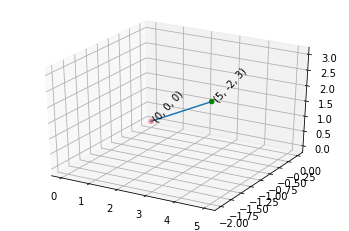
\includegraphics[width = \columnwidth]{./solutions/line_plane/71/Line_Image.png}
    \caption{Line passing through origin and point (5,-2,3)}
    \label{fig:sol_line_plane_71}
\end{figure}
